% -*- Mode:TeX -*-

%% IMPORTANT: The official thesis specifications are available at:
%%            http://libraries.mit.edu/archives/thesis-specs/
%%
%%            Please verify your thesis' formatting and copyright
%%            assignment before submission.  If you notice any
%%            discrepancies between these templates and the 
%%            MIT Libraries' specs, please let us know
%%            by e-mailing thesis@mit.edu

%% The documentclass options along with the pagestyle can be used to generate
%% a technical report, a draft copy, or a regular thesis.  You may need to
%% re-specify the pagestyle after you \include  cover.tex.  For more
%% information, see the first few lines of mitthesis.cls. 

%\documentclass[12pt,vi,twoside]{mitthesis}
%%
%%  If you want your thesis copyright to you instead of MIT, use the
%%  ``vi'' option, as above.
%%
%\documentclass[12pt,twoside,leftblank]{mitthesis}
%%
%% If you want blank pages before new chapters to be labelled ``This
%% Page Intentionally Left Blank'', use the ``leftblank'' option, as
%% above. 

\documentclass[12pt,twoside]{mitthesis}
\usepackage{lgrind}
\usepackage{listings}
\usepackage{listings-golang}
\usepackage{color}
%% These have been added at the request of the MIT Libraries, because
%% some PDF conversions mess up the ligatures.  -LB, 1/22/2014
\usepackage{cmap}
\usepackage[T1]{fontenc}
\pagestyle{plain}

\usepackage{graphicx}
\graphicspath{ {images/} }

\usepackage{hyperref}
\hypersetup{
    colorlinks,
    citecolor=black,
    filecolor=black,
    linkcolor=black,
    urlcolor=black
}
\usepackage{subcaption}
\usepackage{bbding}
%% This bit allows you to either specify only the files which you wish to
%% process, or `all' to process all files which you \include.
%% Krishna Sethuraman (1990).

%\typein [\files]{Enter file names to process, (chap1,chap2 ...), or `all' to
%process all files:}
%\def\all{all}
%\ifx\files\all \typeout{Including all files.} \else \typeout{Including only \files.} \includeonly{\files} \fi

\lstdefinestyle{Golang}{ % add your own preferences
    frame=single,
    basicstyle=\tiny,
    keywordstyle=\color{blue},
    numbers=left,
    %numbersep=5pt,
    showstringspaces=false, 
    stringstyle=\color{blue},
    tabsize=4,
    language=Golang % this is it !
}

\lstset{basicstyle=\tiny, style=Golang}

\begin{document}

% -*-latex-*-
% 
% For questions, comments, concerns or complaints:
% thesis@mit.edu
% 
%
% $Log: cover.tex,v $
% Revision 1.8  2008/05/13 15:02:15  jdreed
% Degree month is June, not May.  Added note about prevdegrees.
% Arthur Smith's title updated
%
% Revision 1.7  2001/02/08 18:53:16  boojum
% changed some \newpages to \cleardoublepages
%
% Revision 1.6  1999/10/21 14:49:31  boojum
% changed comment referring to documentstyle
%
% Revision 1.5  1999/10/21 14:39:04  boojum
% *** empty log message ***
%
% Revision 1.4  1997/04/18  17:54:10  othomas
% added page numbers on abstract and cover, and made 1 abstract
% page the default rather than 2.  (anne hunter tells me this
% is the new institute standard.)
%
% Revision 1.4  1997/04/18  17:54:10  othomas
% added page numbers on abstract and cover, and made 1 abstract
% page the default rather than 2.  (anne hunter tells me this
% is the new institute standard.)
%
% Revision 1.3  93/05/17  17:06:29  starflt
% Added acknowledgements section (suggested by tompalka)
% 
% Revision 1.2  92/04/22  13:13:13  epeisach
% Fixes for 1991 course 6 requirements
% Phrase "and to grant others the right to do so" has been added to 
% permission clause
% Second copy of abstract is not counted as separate pages so numbering works
% out
% 
% Revision 1.1  92/04/22  13:08:20  epeisach

% NOTE:
% These templates make an effort to conform to the MIT Thesis specifications,
% however the specifications can change.  We recommend that you verify the
% layout of your title page with your thesis advisor and/or the MIT 
% Libraries before printing your final copy.
\title{Bootstrapping The Go Runtime For Use On Embedded Systems}

\author{Yanni Coroneos}
% If you wish to list your previous degrees on the cover page, use the 
% previous degrees command:
%       \prevdegrees{A.A., Harvard University (1985)}
% You can use the \\ command to list multiple previous degrees
%       \prevdegrees{B.S., University of California (1978) \\
%                    S.M., Massachusetts Institute of Technology (1981)}
\department{Department of Electrical Engineering and Computer Science}

% If the thesis is for two degrees simultaneously, list them both
% separated by \and like this:
% \degree{Doctor of Philosophy \and Master of Science}
\degree{Master of Engineering in Electrical Engineering and Computer Science}

% As of the 2007-08 academic year, valid degree months are September, 
% February, or June.  The default is June.
\degreemonth{June}
\degreeyear{2017}
\thesisdate{May 18, 2017}

%% By default, the thesis will be copyrighted to MIT.  If you need to copyright
%% the thesis to yourself, just specify the `vi' documentclass option.  If for
%% some reason you want to exactly specify the copyright notice text, you can
%% use the \copyrightnoticetext command.  
%\copyrightnoticetext{\copyright Yanni, 2017.  Do not open till Xmas.}

% If there is more than one supervisor, use the \supervisor command
% once for each.
\supervisor{Dr. Frans Kaashoek}{Charles Piper Professor}

% This is the department committee chairman, not the thesis committee
% chairman.  You should replace this with your Department's Committee
% Chairman.
\chairman{Dr. Christopher Terman}{Chairman, Masters of Engineering Thesis Committee}

% Make the titlepage based on the above information.  If you need
% something special and can't use the standard form, you can specify
% the exact text of the titlepage yourself.  Put it in a titlepage
% environment and leave blank lines where you want vertical space.
% The spaces will be adjusted to fill the entire page.  The dotted
% lines for the signatures are made with the \signature command.
\maketitle

% The abstractpage environment sets up everything on the page except
% the text itself.  The title and other header material are put at the
% top of the page, and the supervisors are listed at the bottom.  A
% new page is begun both before and after.  Of course, an abstract may
% be more than one page itself.  If you need more control over the
% format of the page, you can use the abstract environment, which puts
% the word "Abstract" at the beginning and single spaces its text.

%% You can either \input (*not* \include) your abstract file, or you can put
%% the text of the abstract directly between the \begin{abstractpage} and
%% \end{abstractpage} commands.

% First copy: start a new page, and save the page number.
\cleardoublepage
% Uncomment the next line if you do NOT want a page number on your
% abstract and acknowledgments pages.
% \pagestyle{empty}
\setcounter{savepage}{\thepage}
\begin{abstractpage}
% $Log: abstract.tex,v $
% Revision 1.1  93/05/14  14:56:25  starflt
% Initial revision
% 
% Revision 1.1  90/05/04  10:41:01  lwvanels
% Initial revision
% 
%
%% The text of your abstract and nothing else (other than comments) goes here.
%% It will be single-spaced and the rest of the text that is supposed to go on
%% the abstract page will be generated by the abstractpage environment.  This
%% file should be \input (not \include 'd) from cover.tex.
%%\section{abstract}

Embedded systems are becoming increasingly complicated due to the emergence of
SOCs (system-on-a-chip) with multiple cores, dizzying amounts of peripherals, and
complicated virtual memory systems. Unfortunately, performant embedded systems
for these SOCs are still largely written from scratch in C because heavy
operating systems, such as Linux, can introduce more bugs and degrade real-time
performance.

This thesis proposes a new system called G.E.R.T, the Golang Embedded RunTime,
for multi-core ARM processors.
GERT is a modified version of the Go runtime for
bare-metal operation on multi-core ARMv7a SOC's. It is used to evaluate
the effectiveness of using a high-level, type-safe, and garbage collected
language for embedded applications. G.E.R.T
provides the multiprocessor support and basic memory abstractions of a
typical embedded toolkit while also enabling the user to leverage the language features
of Go in order to develop
concurrent embedded programs that are easier to reason about than similar ones
written in C.


\end{abstractpage}

% Additional copy: start a new page, and reset the page number.  This way,
% the second copy of the abstract is not counted as separate pages.
% Uncomment the next 6 lines if you need two copies of the abstract
% page.
% \setcounter{page}{\thesavepage}
% \begin{abstractpage}
% % $Log: abstract.tex,v $
% Revision 1.1  93/05/14  14:56:25  starflt
% Initial revision
% 
% Revision 1.1  90/05/04  10:41:01  lwvanels
% Initial revision
% 
%
%% The text of your abstract and nothing else (other than comments) goes here.
%% It will be single-spaced and the rest of the text that is supposed to go on
%% the abstract page will be generated by the abstractpage environment.  This
%% file should be \input (not \include 'd) from cover.tex.
%%\section{abstract}

Embedded systems are becoming increasingly complicated due to the emergence of
SOCs (system-on-a-chip) with multiple cores, dizzying amounts of peripherals, and
complicated virtual memory systems. Unfortunately, performant embedded systems
for these SOCs are still largely written from scratch in C because heavy
operating systems, such as Linux, can introduce more bugs and degrade real-time
performance.

This thesis proposes a new system called G.E.R.T, the Golang Embedded RunTime,
for multi-core ARM processors.
GERT is a modified version of the Go runtime for
bare-metal operation on multi-core ARMv7a SOC's. It is used to evaluate
the effectiveness of using a high-level, type-safe, and garbage collected
language for embedded applications. G.E.R.T
provides the multiprocessor support and basic memory abstractions of a
typical embedded toolkit while also enabling the user to leverage the language features
of Go in order to develop
concurrent embedded programs that are easier to reason about than similar ones
written in C.


% \end{abstractpage}

\cleardoublepage

\section*{Acknowledgments}


%%%%%%%%%%%%%%%%%%%%%%%%%%%%%%%%%%%%%%%%%%%%%%%%%%%%%%%%%%%%%%%%%%%%%%
% -*-latex-*-

% Some departments (e.g. 5) require an additional signature page.  See
% signature.tex for more information and uncomment the following line if
% applicable.
% % -*- Mode:TeX -*-
%
% Some departments (e.g. Chemistry) require an additional cover page
% with signatures of the thesis committee.  Please check with your
% thesis advisor or other appropriate person to determine if such a 
% page is required for your thesis.  
%
% If you choose not to use the "titlepage" environment, a \newpage
% commands, and several \vspace{\fill} commands may be necessary to
% achieve the required spacing.  The \signature command is defined in
% the "mitthesis" class
%
% The following sample appears courtesy of Ben Kaduk <kaduk@mit.edu> and
% was used in his June 2012 doctoral thesis in Chemistry. 

\begin{titlepage}
\begin{large}
This doctoral thesis has been examined by a Committee of the Department
of Chemistry as follows:

\signature{Professor Jianshu Cao}{Chairman, Thesis Committee \\
   Professor of Chemistry}

\signature{Professor Troy Van Voorhis}{Thesis Supervisor \\
   Associate Professor of Chemistry}

\signature{Professor Robert W. Field}{Member, Thesis Committee \\
   Haslam and Dewey Professor of Chemistry}
\end{large}
\end{titlepage}


\pagestyle{plain}
  % -*- Mode:TeX -*-
%% This file simply contains the commands that actually generate the table of
%% contents and lists of figures and tables.  You can omit any or all of
%% these files by simply taking out the appropriate command.  For more
%% information on these files, see appendix C.3.3 of the LaTeX manual. 
\tableofcontents
\newpage
\listoffigures
\newpage
\listoftables


%%% This is an example first chapter.  You should put chapter/appendix that you
%% write into a separate file, and add a line \include{yourfilename} to
%% main.tex, where `yourfilename.tex' is the name of the chapter/appendix file.
%% You can process specific files by typing their names in at the 
%% \files=
%% prompt when you run the file main.tex through LaTeX.
\chapter{Introduction}

Micro-optimization is a technique to reduce the overall operation count of
floating point operations.  In a standard floating point unit, floating
point operations are fairly high level, such as ``multiply'' and ``add'';
in a micro floating point unit ($\mu$FPU), these have been broken down into
their constituent low-level floating point operations on the mantissas and
exponents of the floating point numbers.

Chapter two describes the architecture of the $\mu$FPU unit, and the
motivations for the design decisions made.

Chapter three describes the design of the compiler, as well as how the
optimizations discussed in section~\ref{ch1:opts} were implemented.

Chapter four describes the purpose of test code that was compiled, and which
statistics were gathered by running it through the simulator.  The purpose
is to measure what effect the micro-optimizations had, compared to
unoptimized code.  Possible future expansions to the project are also
discussed.

\section{Motivations for micro-optimization}

The idea of micro-optimization is motivated by the recent trends in computer
architecture towards low-level parallelism and small, pipelineable
instruction sets \cite{patterson:risc,rad83}.  By getting rid of more
complex instructions and concentrating on optimizing frequently used
instructions, substantial increases in performance were realized.

Another important motivation was the trend towards placing more of the
burden of performance on the compiler.  Many of the new architectures depend
on an intelligent, optimizing compiler in order to realize anywhere near
their peak performance
\cite{ellis:bulldog,pet87,coutant:precision-compilers}.  In these cases, the
compiler not only is responsible for faithfully generating native code to
match the source language, but also must be aware of instruction latencies,
delayed branches, pipeline stages, and a multitude of other factors in order
to generate fast code \cite{gib86}.

Taking these ideas one step further, it seems that the floating point
operations that are normally single, large instructions can be further broken
down into smaller, simpler, faster instructions, with more control in the
compiler and less in the hardware.  This is the idea behind a
micro-optimizing FPU; break the floating point instructions down into their
basic components and use a small, fast implementation, with a large part of
the burden of hardware allocation and optimization shifted towards
compile-time.

Along with the hardware speedups possible by using a $\mu$FPU, there are
also optimizations that the compiler can perform on the code that is
generated.  In a normal sequence of floating point operations, there are
many hidden redundancies that can be eliminated by allowing the compiler to
control the floating point operations down to their lowest level.  These
optimizations are described in detail in section~\ref{ch1:opts}.

\section{Description of micro-optimization}\label{ch1:opts}

In order to perform a sequence of floating point operations, a normal FPU
performs many redundant internal shifts and normalizations in the process of
performing a sequence of operations.  However, if a compiler can
decompose the floating point operations it needs down to the lowest level,
it then can optimize away many of these redundant operations.  

If there is some additional hardware support specifically for
micro-optimization, there are additional optimizations that can be
performed.  This hardware support entails extra ``guard bits'' on the
standard floating point formats, to allow several unnormalized operations to
be performed in a row without the loss information\footnote{A description of
the floating point format used is shown in figures~\ref{exponent-format}
and~\ref{mantissa-format}.}.  A discussion of the mathematics behind
unnormalized arithmetic is in appendix~\ref{unnorm-math}.

The optimizations that the compiler can perform fall into several categories:

\subsection{Post Multiply Normalization}

When more than two multiplications are performed in a row, the intermediate
normalization of the results between multiplications can be eliminated.
This is because with each multiplication, the mantissa can become
denormalized by at most one bit.  If there are guard bits on the mantissas
to prevent bits from ``falling off'' the end during multiplications, the
normalization can be postponed until after a sequence of several
multiplies\footnote{Using unnormalized numbers for math is not a new idea; a
good example of it is the Control Data CDC 6600, designed by Seymour Cray.
\cite{thornton:cdc6600} The CDC 6600 had all of its instructions performing
unnormalized arithmetic, with a separate {\tt NORMALIZE} instruction.}.

% This is an example of how you would use tgrind to include an example
% of source code; it is commented out in this template since the code
% example file does not exist.  To use it, you need to remove the '%' on the
% beginning of the line, and insert your own information in the call.
%
%\tagrind[htbp]{code/pmn.s.tex}{Post Multiply Normalization}{opt:pmn}

As you can see, the intermediate results can be multiplied together, with no
need for intermediate normalizations due to the guard bit.  It is only at
the end of the operation that the normalization must be performed, in order
to get it into a format suitable for storing in memory\footnote{Note that
for purposed of clarity, the pipeline delays were considered to be 0, and
the branches were not delayed.}.

\subsection{Block Exponent}

In a unoptimized sequence of additions, the sequence of operations is as
follows for each pair of numbers ($m_1$,$e_1$) and ($m_2$,$e_2$).
\begin{enumerate}
  \item Compare $e_1$ and $e_2$.
  \item Shift the mantissa associated with the smaller exponent $|e_1-e_2|$
        places to the right.
  \item Add $m_1$ and $m_2$.
  \item Find the first one in the resulting mantissa.
  \item Shift the resulting mantissa so that normalized
  \item Adjust the exponent accordingly.
\end{enumerate}

Out of 6 steps, only one is the actual addition, and the rest are involved
in aligning the mantissas prior to the add, and then normalizing the result
afterward.  In the block exponent optimization, the largest mantissa is
found to start with, and all the mantissa's shifted before any additions
take place.  Once the mantissas have been shifted, the additions can take
place one after another\footnote{This requires that for n consecutive
additions, there are $\log_{2}n$ high guard bits to prevent overflow.  In
the $\mu$FPU, there are 3 guard bits, making up to 8 consecutive additions
possible.}.  An example of the Block Exponent optimization on the expression
X = A + B + C is given in figure~\ref{opt:be}.

% This is an example of how you would use tgrind to include an example
% of source code; it is commented out in this template since the code
% example file does not exist.  To use it, you need to remove the '%' on the
% beginning of the line, and insert your own information in the call.
%
%\tgrind[htbp]{code/be.s.tex}{Block Exponent}{opt:be}

\section{Integer optimizations}

As well as the floating point optimizations described above, there are
also integer optimizations that can be used in the $\mu$FPU.  In concert
with the floating point optimizations, these can provide a significant
speedup.  

\subsection{Conversion to fixed point}

Integer operations are much faster than floating point operations; if it is
possible to replace floating point operations with fixed point operations,
this would provide a significant increase in speed.

This conversion can either take place automatically or or based on a
specific request from the programmer.  To do this automatically, the
compiler must either be very smart, or play fast and loose with the accuracy
and precision of the programmer's variables.  To be ``smart'', the computer
must track the ranges of all the floating point variables through the
program, and then see if there are any potential candidates for conversion
to floating point.  This technique is discussed further in
section~\ref{range-tracking}, where it was implemented.

The other way to do this is to rely on specific hints from the programmer
that a certain value will only assume a specific range, and that only a
specific precision is desired.  This is somewhat more taxing on the
programmer, in that he has to know the ranges that his values will take at
declaration time (something normally abstracted away), but it does provide
the opportunity for fine-tuning already working code.

Potential applications of this would be simulation programs, where the
variable represents some physical quantity; the constraints of the physical
system may provide bounds on the range the variable can take.
\subsection{Small Constant Multiplications}

One other class of optimizations that can be done is to replace
multiplications by small integer constants into some combination of
additions and shifts.  Addition and shifting can be significantly faster
than multiplication.  This is done by using some combination of
\begin{eqnarray*}
a_i & = & a_j + a_k \\
a_i & = & 2a_j + a_k \\
a_i & = & 4a_j + a_k \\
a_i & = & 8a_j + a_k \\
a_i & = & a_j - a_k \\
a_i & = & a_j \ll m \mbox{shift}
\end{eqnarray*}
instead of the multiplication.  For example, to multiply $s$ by 10 and store
the result in $r$, you could use:
\begin{eqnarray*}
r & = & 4s + s\\
r & = & r + r
\end{eqnarray*}
Or by 59:
\begin{eqnarray*}
t & = & 2s + s \\
r & = & 2t + s \\
r & = & 8r + t
\end{eqnarray*}
Similar combinations can be found for almost all of the smaller
integers\footnote{This optimization is only an ``optimization'', of course,
when the amount of time spent on the shifts and adds is less than the time
that would be spent doing the multiplication.  Since the time costs of these
operations are known to the compiler in order for it to do scheduling, it is
easy for the compiler to determine when this optimization is worth using.}.
\cite{magenheimer:precision}

\section{Other optimizations}

\subsection{Low-level parallelism}

The current trend is towards duplicating hardware at the lowest level to
provide parallelism\footnote{This can been seen in the i860; floating point
additions and multiplications can proceed at the same time, and the RISC
core be moving data in and out of the floating point registers and providing
flow control at the same time the floating point units are active. \cite{byte:i860}}

Conceptually, it is easy to take advantage to low-level parallelism in the
instruction stream by simply adding more functional units to the $\mu$FPU,
widening the instruction word to control them, and then scheduling as many
operations to take place at one time as possible.

However, simply adding more functional units can only be done so many times;
there is only a limited amount of parallelism directly available in the
instruction stream, and without it, much of the extra resources will go to
waste.  One process used to make more instructions potentially schedulable
at any given time is ``trace scheduling''.  This technique originated in the
Bulldog compiler for the original VLIW machine, the ELI-512.
\cite{ellis:bulldog,colwell:vliw}  In trace scheduling, code can be
scheduled through many basic blocks at one time, following a single
potential ``trace'' of program execution.  In this way, instructions that
{\em might\/} be executed depending on a conditional branch further down in
the instruction stream are scheduled, allowing an increase in the potential
parallelism.  To account for the cases where the expected branch wasn't
taken, correction code is inserted after the branches to undo the effects of
any prematurely executed instructions.

\subsection{Pipeline optimizations}

In addition to having operations going on in parallel across functional
units, it is also typical to have several operations in various stages of
completion in each unit.  This pipelining allows the throughput of the
functional units to be increased, with no increase in latency.

There are several ways pipelined operations can be optimized.  On the
hardware side, support can be added to allow data to be recirculated back
into the beginning of the pipeline from the end, saving a trip through the
registers.  On the software side, the compiler can utilize several tricks to
try to fill up as many of the pipeline delay slots as possible, as
seendescribed by Gibbons. \cite{gib86}




\chapter{Introduction}

Modern embedded systems are composed of multicore SOCs that require
careful thought about concurrency. C is the
most commonly used language to program such low level systems because
it is simple and expressive, but it is
a double-edged blade. Low level code written in C can more easily and
directly interface with hardware, but it can also be plagued with
difficult bugs, especially concurrency-related bugs and memory bugs like
use after free.

Concurrent, high-level user space programs that do not directly interface with
hardware, on the other hand, are usually written in a
high-level language, such as Rust or Go, which abstracts concurrency
and provides memory safety. Rust, Go, and other High Level Languages (HLL's)
will usually ensure that there is never an out of bounds error, use
after free error, or unsafe cast. HLL's can also provide native concurrency
support through primitives like channels. The downsides of HLLs is that those
nice featues come at a cost of garbage collection and many runtime checks.
Despite the shortcomings, HLLs are still preferred to C programs because fast,
modern computers negate the performance cost. Now that embedded devices are also very fast,
the possibility of using a HLL on a performant embedded system is attractive.

Embedded programmers are often drawn towards using Linux for their work
because then they can write their embedded program in user space with a
high level language in order to avoid the difficulty and poor concurrency
support of C. Popular platforms that use this paradigm include
the Raspi and Beaglebone. However, embedded programs that run in user space suffer
from significant event latency because external interrupts
must shuffle their way through the kernel. Additionally, the kernel's scheduler
will also constantly preempt the program. This performance loss is compounded by the
performance penalties that HLL's also impose on programs.
Usually, an experienced programmer does not even want or need the
kernel, but they pay the price just to run the high-level embedded code.

Traditional operating systems impose expensive and redundant checks on
high-level programs. For example,
Go already ensures that different threads cannot access each other's memory and that null pointers
will not be dereferenced. The OS is intended to work with buggy C programs though, so it must still switch
page tables when switching processes and be prepared for page faults when bad accesses occur. This machinery
is expensive and redundant for programs written in a HLL. Since embedded applications only run a single
program, it is possible to completely do away with the OS underneath a high-level program and regain the
lost performance without any degredation in safety.

There are ongoing efforts to bring high-level languages to desktop
operating system kernels and also single-core microcontrollers, but
there is no known system which provides a high-level language environment for
multicore SOCs. Singularity <cite> and Biscuit <cite> are desktop
operating system kernels, written in Sing\# and Go, which focus on
hosting user-space programs. Copper <cite> and MicroPython <cite>
are small embedded toolkits, written in Rust and Python, which aim
to provide a high-level programming environment for single-core
microcontrollers. Multicore SOCs have, so far, been left out of the
picture. This thesis presents a new embedded toolkit, the Golang Embedded
RunTime (GERT), which is specifically intended for concurrent, bare-metal embedded applications.

\section{Outline}
Below is an outline of this thesis.
\begin{itemize}
  \item Chapter 2 explains why Go was chosen for GERT and also the basic intuition behind the Go runtime implementation
  \item Chapter 3 presents the core work of this thesis, or how the runtime was modified to work on bare metal
  \item Chapter 4 shows how to use GERT, an essential aspect of any toolkit
  \item Chapter 5 evaluates GERT on embedded benchmarks and also two embedded case studies
  \item Chapter 6 concludes this thesis with a crystalization of the results and their implication
\end{itemize}

\chapter{Introduction}

Modern embedded systems are composed of multicore SOCs that require
careful thought about concurrency. C is the
most commonly used language to program such low level systems because
it is simple and expressive, but it is
a double-edged blade. Low level code written in C can more easily and
directly interface with hardware, but it can also be plagued with
difficult bugs, especially concurrency-related bugs and memory bugs like
use after free.

Concurrent, high-level user space programs that do not directly interface with
hardware, on the other hand, are usually written in a
high-level language, such as Rust or Go, which abstracts concurrency
and provides memory safety. Rust, Go, and other High Level Languages (HLL's)
will usually ensure that there is never an out of bounds error, use
after free error, or unsafe cast. HLL's can also provide native concurrency
support through primitives like channels. The downsides of HLLs is that those
nice featues come at a cost of garbage collection and many runtime checks.
Despite the shortcomings, HLLs are gaining widespread use because computers,
in general, are getting faster. Now that embedded devices are also very fast,
the possibility of using an HLL on a performant embedded system is undeniable.

Embedded programmers are often drawn towards using Linux for their work
because then they can write their embedded program in user space with a
high level language in order to avoid the difficulty and poor concurrency
support of C. Popular platforms that use this paradigm include
the Raspi and Beaglebone. However, embedded programs that run in user space suffer
from significant event latency because external interrupts
must shuffle their way through the kernel. Additionally, the kernel's scheduler
will also constantly preempt the program. This performance loss is compounded by the
performance penalties that HLL's also impose on programs.
Usually, an experienced programmer does not even want or need the
kernel, but they pay the price just to run the high-level embedded code.

There are ongoing efforts to bring high-level languages to desktop
operating system kernels and also single-core microcontrollers, but
there is no known system which provides a high-level language environment for
multicore SOCs. Singularity <cite> and Biscuit <cite> are desktop
operating system kernels, written in Sing\# and Go, which focus on
hosting user-space programs. Copper <cite> and MicroPython <cite>
are small embedded toolkits, written in Rust and Python, which aim
to provide a high-level programming environment for single-core
microcontrollers. Multicore SOCs have, so far, been left out of the
picture. This thesis presents a new embedded toolkit, GERT, which
is specifically intended for concurrent, bare-metal embedded applications.

GERT is a bare-metal, Go-based embedded toolkit for multicore ARMv7a processors.
It was developed in order to make bare-metal programming
easier for ARMv7a SOCs with the help of Go's channels, goroutines, and isolation.
G.E.R.T can run on a single-core processor but its effectiveness is substantially
reduced because any blocking operation can lock the whole system. On the other hand,
G.E.R.T will automatically scale to utilize all available cpus in multicore systems
because the Go runtime automatically scales to all available cpus. GERT is not intended
to outperform bare-metal C, but rather to provide isolation and native concurrency
support in a bare-metal environment.

One particular concern about using a garbage-collected language, such as Go,
for low-level code is GC pause times. In Linux, a GC pause prevents the program from
responding to any input and producing any output; the program is literally paused.
GERT gets around this issue by allowing interrupt handlers to execute even when the
world is stopped due to a garbage collection. The only caveat is that interrupt handlers
cannot contain blocking operations because then execution could funnel into the Go scheduler
and lead to a catastrophe.

\section{Why Write Low Level System Code in Go?}

At first glance, Go code looks a lot like C. There are no
classes and every object has a type which is known at compile time.
This already makes Go a good systems language, but Go's
greatest feature is its built-in support for concurrency through
goroutines and channels. Goroutines are lightweight threads that
the Go runtime can schedule without help from the operating system.
Channels are typed FIFO queues which can help to serialize
asynchronous events, perhaps coming from several goroutines.
With these features, Go is like an updated version
of C for multicore systems, but without buffer overflows and
null pointer dereferences.

Go's implementation mirrors that of a small
real-time OS. Go's threads are lightweight and
cooperatively scheduled so that execution only transfers during
blocking operations. The runtime also manages its own pool of memory
and exports its own atomic primitives through the standard "sync"
package. In fact, Go provides most of the common OS primitives natively
in its standard libraries <https://golang.org/pkg/\#stdlib>. This means
that G.E.R.T can also provide most of the convenience of a full-blown kernel
without latency degredation.

Embedded systems are increasingly relying on dedicated peripherals to
provide service, instead of very fast cpus. SOCs contain dedicated
silicon peripherals to help with everything from serial communication to
interrupt priority filtering. These peripherals free the cpus from bit-banging
high-frequency signals so they can spend more time directing program
flow instead. Go fits in well with such a system because its goroutines can be
used to concurrently monitor state and channels can be used to relay that information
back to a central coordinator. When an output must be switched, G.E.R.T simply
issues a driver call that changes the behavior of a peripheral.

\section{Outline}
Outline the rest of the thesis

%Stay tuned!
%Modern embedded systems are composed of multicore SOCs that require
%careful thought about race conditions and event serialization. Like
%operating system kernels, most of these embedded systems are still implemented
%in C because it is a simplistic language that makes it good for "bare-metal"
%development.
%
%
%outline:
%computers are quicker and multicore programming is scary, but everyone still uses C
%
%C's simplicity makes it error prone for concurrent programs.
%Because C is very simple, the programmer must implement additional complexities in order to write
%concurrent programs.
%
%try2:
%Low-level system code has been written in C since the 1970's because it is powerful
%and reliable. C can be used to express any operation a computer can do and it can also be
%compiled to fast byte code. Once, during an interview, an engineer even remarked: "If you
%can't do it in C, you can't do it". This does not mean that C is always the best choice though.
%
%Even though multicore systems are commonplace now, kernels are still written in C.
%
%Writing complex concurrent programs in C is too hard. Because C is very simple,
%the programmer must implement additional complexities in order to write
%concurrent programs.
%
%
%There are very
%few built-in abstractions so it is left to the programmer to layer additional complexities
%in order to accomplish a task.
%
%
%try 1:
%Low-level system code has been written in C since the 1970's because C is powerful
%and reliable. C can be used to express any operation a computer can do and it doesn't come
%with any baggage like languages with a runtime do. C is also easy to learn because it doesn't
%require advanced degrees in order to comprehend, like Haskell and Coq do. The problems with C
%only begin to show when concurrency comes into play. C, by itself, has no idea of concurrency
%or concurrent programming patterns. It is really all up to the programmer to lay down these
%abstractions. Combined with the burden of manual memory management, concurrent programming in C
%almost always results in pouring over JTAG trace logs for hints of a race condition.
%  Faced with this bleak outlook, perhaps it is reasonable to take a performance hit in exchange for
%faster development and less bugs. After all, computers have gotten significantly quicker in
%the last 20 years. This is where Go can come in. Go is meant to be a systems language
%that provides fundamental support for concurrency and cummincation

\chapter{The Go Runtime On Bare Metal}

\begin{figure}[h]
\begin{center}
  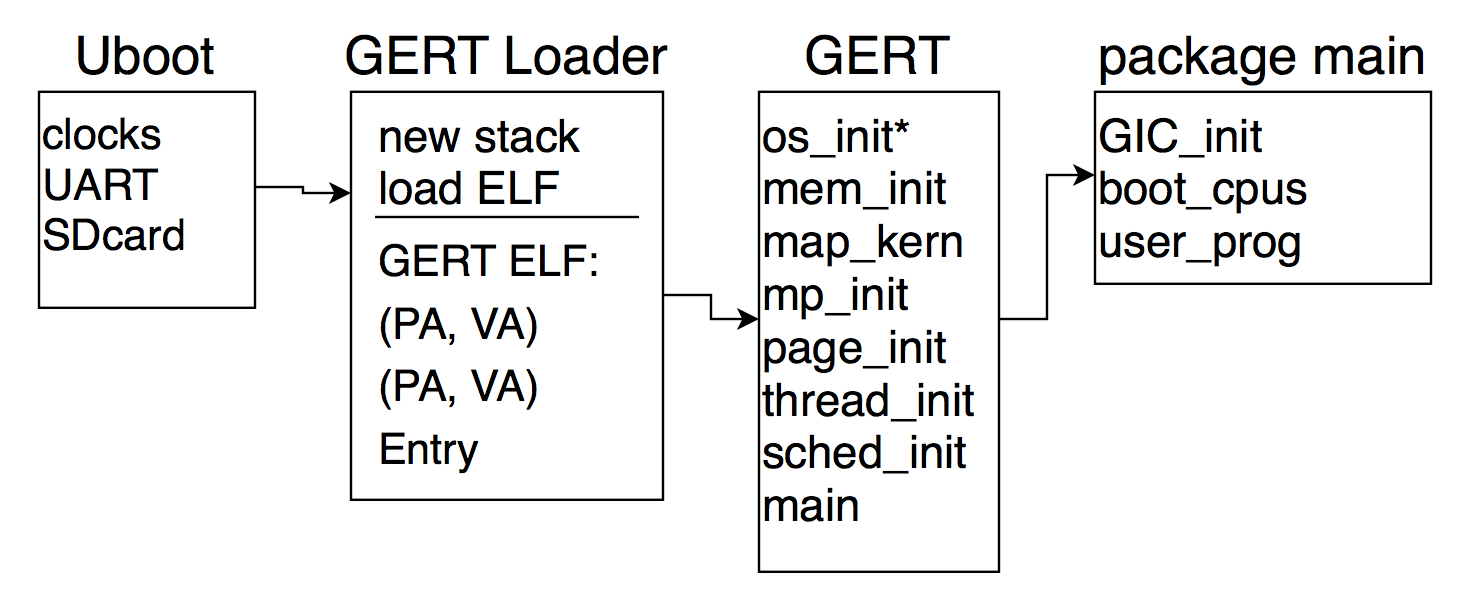
\includegraphics[scale=0.5]{boot_process}
\end{center}
  \caption{GERT Boot Process. * means performed by the Go runtime} \label{fig:boot}
\end{figure}

Even though Go code is compiled, it relies on a runtime to coordinate certain actions with the OS and support its concurrency model.
Timers, locks, and file descriptors are just a few of the OS abstractions that the runtime hinges on
in order to function at all. This means that getting compiled Go code to run bare metal on an SOC requires
more than just a boot loader, the Go runtime itself must be modified to work without any OS abstractions.
This poses a bootstrapping problem because any modifications made to the Go runtime's initialization
process must not inadvertently cause it to use an abstraction that does not yet exist. For example,
creating a new object with $make()$ \footnote{In Go, new objects are created with \textit{make}} during the boot process would be disastrous if the GC has not yet been initialized.
Modifying the Go runtime to boot on bare metal is tricky process because all additions should be made
in a non-destructive way that still preserves all of Go's useful primitives, including the standard library.


In observation of these constraints, GERT boots via a 3-step process as shown in figure \ref{fig:boot}.
In step 1, u-boot is used to set up device clocks and load the code for step 2 off of an SD card. Step 2 prepares the
Go stack with arguments and environment variables before jumping into GERT. Step 3 runs inside of GERT and it
finishes the boot process by initializing virtual memory, threading, and interrupt handlers.


%%The first stage is the u-boot
%%bootloader, a common bootloader for embedded devices, which
%%configures the clocks and loads the second stage off of an SD card. The second
%%stage bootloader is a small C program which contains the entire GERT kernel ELF in its data section. This stage sets
%%up the inital Go stack and loads the GERT ELF into memory before jumping to its entry point. The third stage
%%of the bootloader lives inside GERT and is mostly written in Go, along with some Plan 9 assembly. It finishes the
%%boot process by initializing virtual memory, threading, and additional cpus.



%%Working off the
%%initial stack from stage 2, the stage 3 bootloader enumerates all of RAM into page tables and creates an idenity mapping
%%with a new stack before turning on the MMU. After this, a thread scheduler is setup and synchronization primitives, like
%%$futex()$ are enabled. Additional CPU's are booted in main after the Go runtime has finished initializing.

%%\section{System Specification}
%%GERT is written on a Freescale i.MX6 Quad SOC which implements the (32 bit) ARMv7a Cortex A9 MPCore architecture.
%%The SOC sits on a Wandboard Quad baseboard. The i.MX6 Quad has 2GB of RAM and a wealth of memory mapped peripherals.
%%Look at the memory map below. The rest of this chapter will discuss the implementation details of booting and
%%running the Go runtime bare-metal on this SOC.
%%
%%<memory map of imx6 here>
%%
%%<memory map of GERT here>

\section{Step 1 Bring Up}
Unlike desktop PCs, SOCs have no BIOS, so it is entirely the programmer's job to initialize device clocks
and power on essential peripherals like the memory controller. U-boot is a simple bootloader which abstracts
this laborious process for all of the SOCs which it supports. GERT uses it to chain load its own, more specialized,
bootloader. The u-boot loader is used to initialize device clocks and execute the GERT bootloader.


%%When the SOC is powered on, the program counter starts executing from ROM. The code in the ROM reads
%%u-boot into RAM and jumps into it. Unlike desktop PCs and laptops which use a BIOS to configure the
%%frequency dividers and RAM timings, the iMX6 has no such thing so u-boot does it instead.
%%U-boot programs the myriad of frequency dividers which are required
%%to run the i.MX6 at a frequency of 792MHz per core. After this, u-boot loads the GERT
%%kernel off the sdcard and into RAM at address 0x50000000. This address is specifically chosen because it
%%does not overlap with any ELF program headers of the GERT kernel which are loaded in stage 2. After
%%the stage 2 bootloader is in RAM, uboot jumps into it.

\section{Step 2 GERT Kernel Installation}
The GERT loader is a C program which sets up the initial Go stack and decompresses the Go kernel
ELF into RAM. GERT is compiled as a Linux Go program, so the Go runtime expects to find arguments
and environment variables in its initial stack. This is a convenient channel for passing
information; for example, the GERT loader uses this to pass the size of the GERT kernel.
GERT later uses this size to determine its location in memory and initialize virtual memory.

The link address of the GERT binary must be also adjusted on a per-SOC basis in order for the Go
runtime to avoid using inaccessible memory. By default, Go compiler links and loads at 0x0. This is incorrect
for most SOCs because they have reserved regions near that address. Fortunately, the Go compiler can
generate code at a different link addresses by passing in a link-time flag, so this is not a significant problem.

%%Much like Linux, the kernel of GERT is wrapped in a custom
%%bootloader. This is necessary because GERT is compiled as a user space
%%Linux program which expects a stack and the standard ELF auxiliary vectors to be present on
%%startup.
%%
%%By default, the Go compiler links all programs at address 0x0. This would normally
%%be a disaster for the i.MX6 because the first megabyte of RAM is either inaccessable
%%or reserved for peripherals. One solution around this is to simply turn on the MMU
%%in the stage 2 bootloader but this creates a headache with preserving page tables
%%across the transition to Go. An alternative, and much simpler, solution is to
%%just change the link address of the Go ELF. This is the preferred approach so
%%GERT's build system uses a link address of 0x10000000 for the Go runtime, which is the start of
%%RAM on the iMX6. After loading the Go binary into RAM, the stage 2 bootloader reserves
%%4kb of initial stack and jumps into GERT.


\section{Step 3 Go Runtime Setup}

The Go runtime forms the basis of GERT's functionality but it is not equipped to
run on bare metal. The final steps of the boot process are accomplished in Go. GERT
initializes the minimum set of OS abstractions
to be used by the Go runtime, before the runtime actually uses them. These abstractions are
virtual memory, thread scheduling, interrupt handling, timers, and booting secondary cores.

%%The thread scheduler and virtual memory system are statically initialized
%%in order to prevent Go runtime subsystems from running before the environment
%%is ready. At the beginning of execution, GERT is in a constrained
%%situation: Linux is not there but the Go runtime thinks it is. Specifically, there
%%is no scheduler, no virtual memory, no syscalls. Nothing but a 4kb stack
%%and the program counter. This is clearly inadequate for the Go runtime
%%to do anything but crash, so GERT creates all of these missing subsystems
%%,in Go, before the runtime actually uses them.


\subsection{Virtual Memory Setup}
\begin{figure}[h]
  \begin{subfigure}[t!]{0.5\textwidth}
 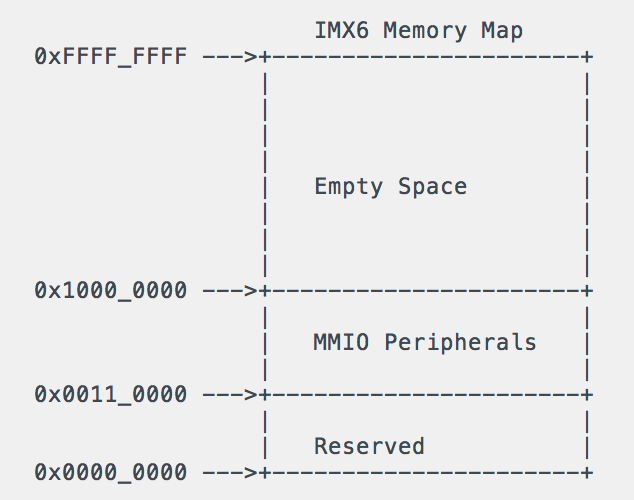
\includegraphics[scale=0.6]{imxmap}
  \end{subfigure}
  \begin{subfigure}[t!]{0.5\textwidth}
 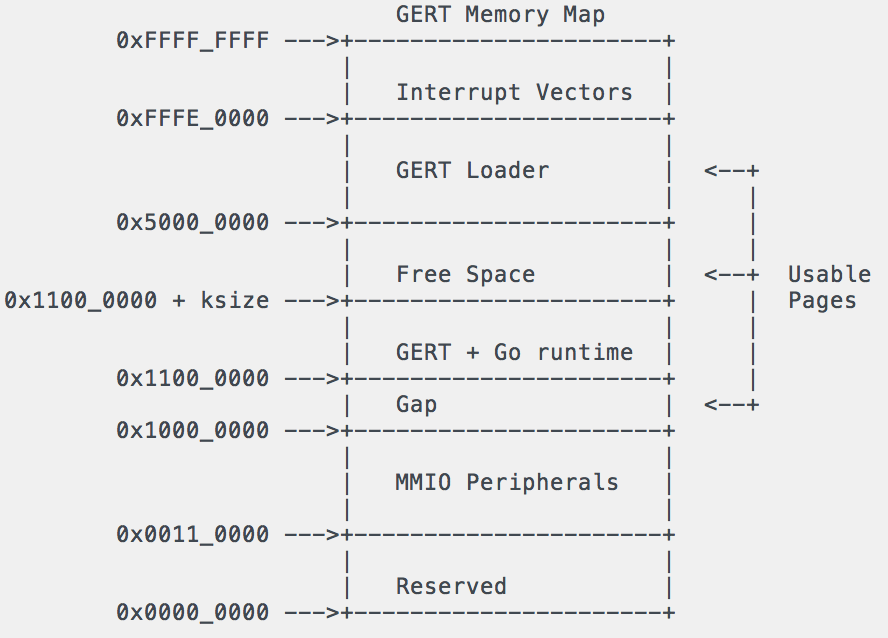
\includegraphics[scale=0.5]{gertmap}
  \end{subfigure}
  \caption{Memory Map Before and After Boot} \label{fig:gertmap}
\end{figure}

GERT needs to have virtual memory enabled so the Go runtime can function properly and so
GERT can manage available memory. Fig. \ref{fig:gertmap} shows the physical memory map
of an i.MX6 SOC before GERT is booted and after GERT has booted.
Even though the
runtime is linked at a high address, Go still requests memory inside the reserved regions of physical
memory so a virtual address must be mapped there. GERT also uses paging to create a virtually contiguous
address space which is easier to manage than a physically discontiguous address space. For example,
the Go runtime sometimes requests large chunks of continuous memory. It is possible that there is not
a large enough chunk of physical memory to return due to fragmentation of MMIO peripherals, but there
will be a big enough chunk in virtual memory. GERT also recycles the bootloader using virtual
memory by simply marking its occupied area as usable pages.

GERT uses 1MB page tables and it rarely has to reload them. GERT has no userspace or programs
that must be isolated from each other and the Go runtime only allocates memory infrequently
and in large chunks. This is the only time that GERT has to reload the page tables.
This static nature of GERT's memory space means that 4kb pages are unnecessary
and even costly because they incur a 2-level page translation \footnote{4kb paging in ARMv7a requires $2^11=4096$ entries in the L1 table and $2^8=256$ entries in each L2 table} , unlike 1MB pages which just require
a 1-level walk. By the time user code starts running in GERT, the runtime has nearly completed
all of its memory manipulation.

\subsection{Thread Scheduling and Trapframes}
\begin{figure}[h]
\begin{center}
  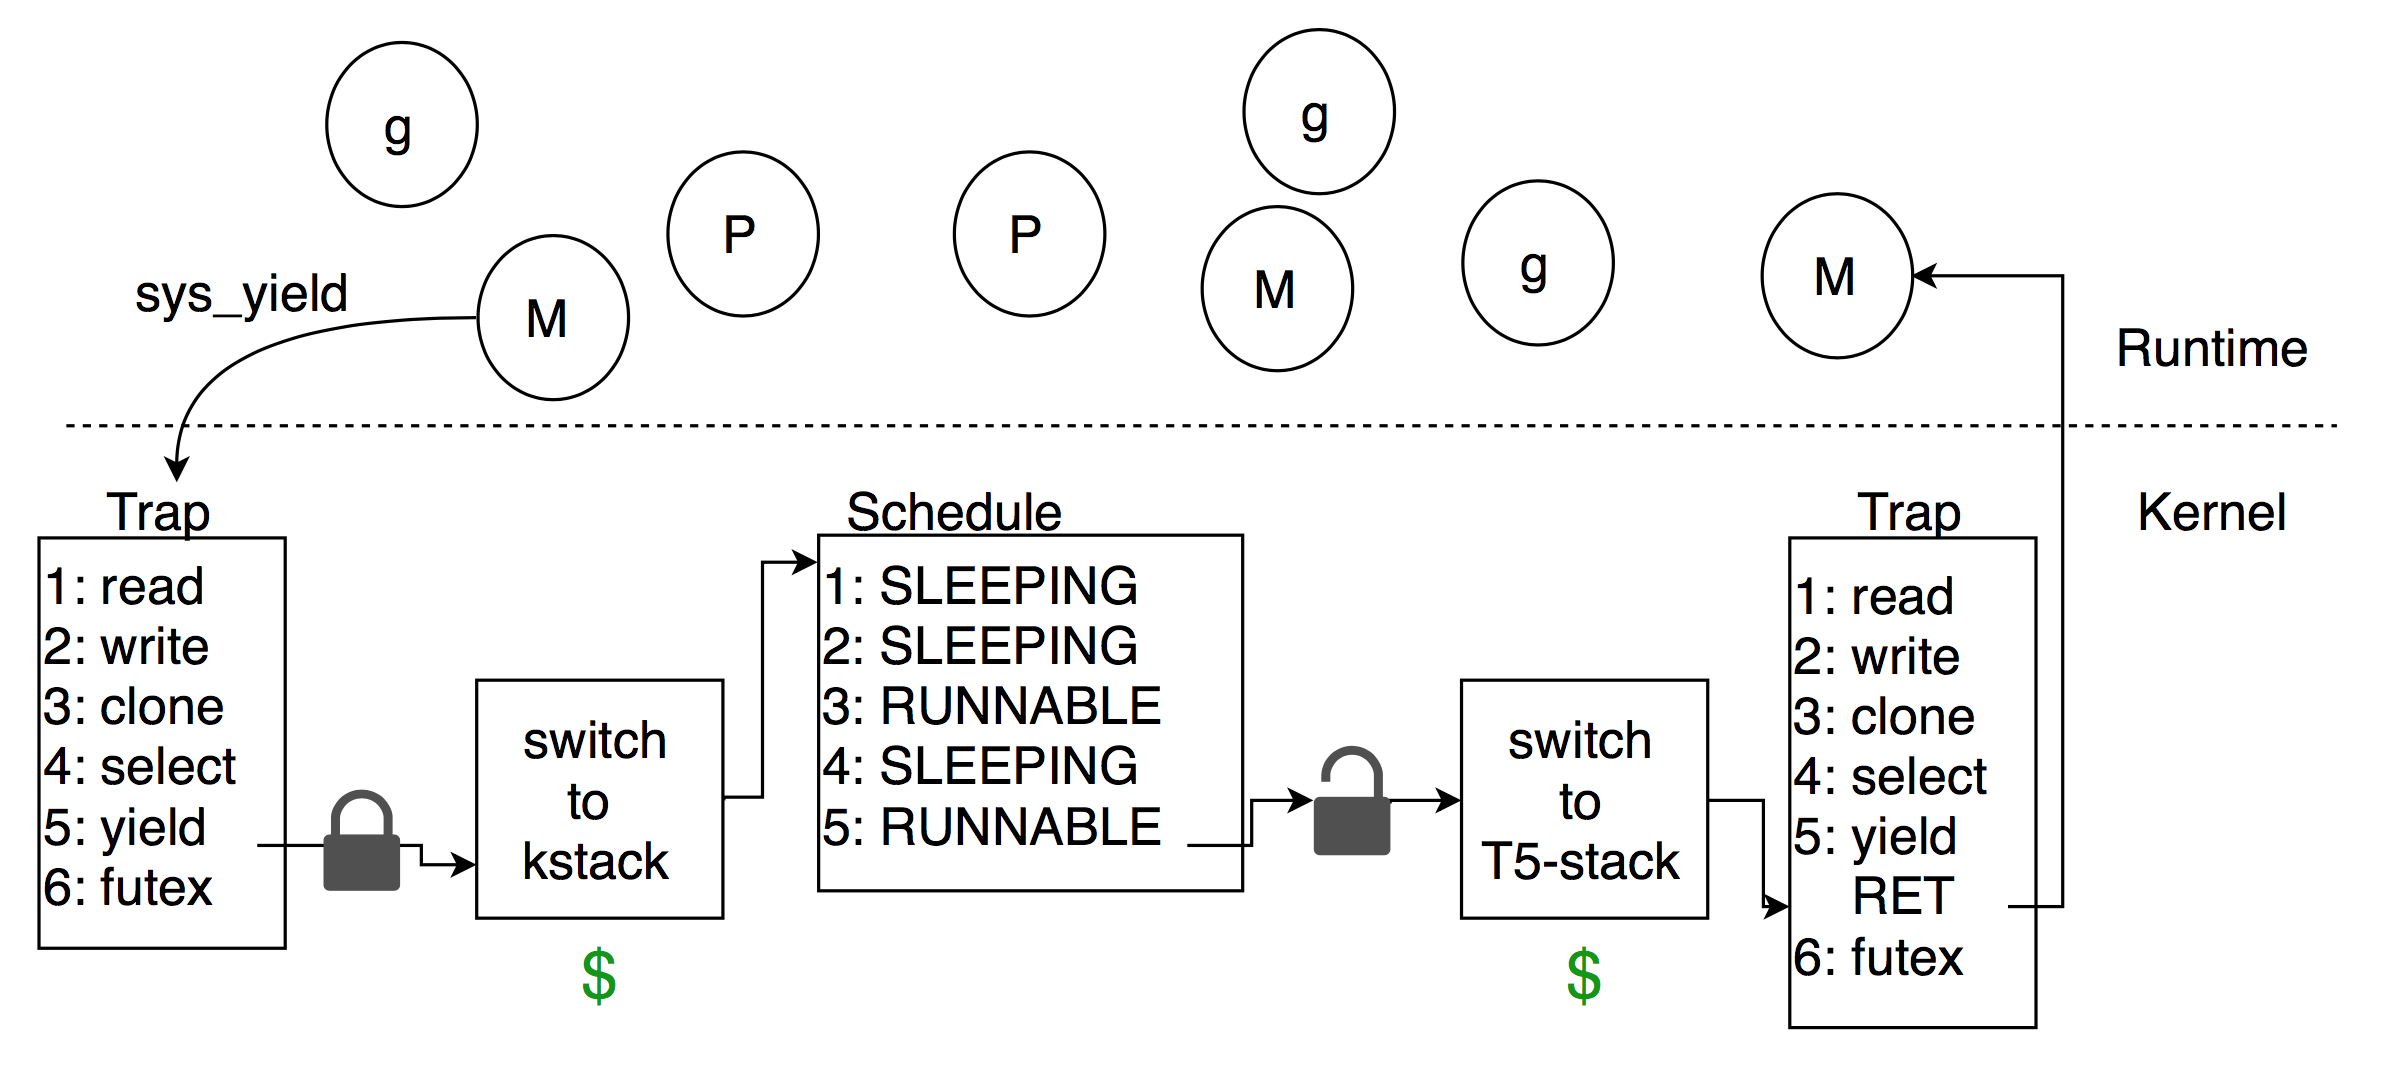
\includegraphics[scale=0.25]{syscall}
\end{center}
  \caption{Handling Go Runtime Syscalls} \label{fig:syscall}
\end{figure}

GERT models the entire Go runtime as a black box whose only entry and exit points
are through the syscalls it makes. This model is shown in \ref{fig:syscall} along with the
control flow of \textit{sys\_yield}, which invokes the GERT scheduler. To be clear, there is no such thing as a syscall in GERT;
it is a single-address space application that runs in privileged mode.
Whenever the Go runtime makes a syscall, the processor mode is not changed and a new page table
is not installed. Instead, every instance of the syscall instruction in the Go runtime has been
replaced with a function call to $trap$, the entry point into the GERT kernel.
While execution is in $trap$, the Go runtime believes
that the OS is servicing its syscall, but in actuality the blocked thread is still running Go code inside
the GERT kernel. The list of Linux syscalls that has to be re-implemented is shown in fig. \ref{fig:syscalls}.
All syscalls with an * are expensive because they cause a stack switch to the scheduler's stack.


\begin{figure} [h]
\begin{center}
  \begin{tabular}{ | l | l |}
    \hline
    Syscall & Used For \\ \hline
    exit & crash \\ \hline
    read & read from a file descriptor. All reads go to UART\\ \hline
    write & write to a file descriptor. All writes go to UART\\ \hline
    clone & spawn a new M\\ \hline
    *select & blocking read operation\\ \hline
    *yield & yield to scheduler\\ \hline
    mmap & allocate large chunks of memory\\ \hline
    *futex & wait for a condition to become true\\ \hline
    clock\_gettime & goroutine scheduling and time package\\ \hline
    getpid & runtime asks its pid\\ \hline
  \end{tabular}
\end{center}
  \caption{Linux Syscalls That Are Re-implemented in GERT. * means syscall causes stack switch}  \label{fig:syscalls}
\end{figure}

GERT also maintains data structures that track the state of Go threads
outside the runtime's knowledge. It is important that all state inside the GERT kernel is
allocated outside the Go runtime's knowledge either with global variables or the kernel's
static memory allocator. If this constraint is not observed, then it is possible for the garbage collector
to potentially recycle memory from the kernel.

Each thread in GERT has an id, status, futex address, and trapframe associated with it (\ref{fig:threadtrap}).
The trapframe records the state of all the registers and the location of the stack at
the time that the Go runtime made a syscall.

\begin{figure}[h]
  \begin{lstlisting}
type thread_t struct {
	tf       trapframe
	state    uint32
	futaddr  uintptr
	sleeptil timespec
	id       uint32
}
type trapframe struct {
	lr  uintptr
	sp  uintptr
	fp  uintptr
	r0  uint32
	r1  uint32
	r2  uint32
	r3  uint32
	r10 uint32
}
\end{lstlisting}

  \caption{Thread state and Trapframes} \label{fig:threadtrap}
\end{figure}

When threads go to sleep, the CPU stores their execution context in a trapframe.
When a thread is scheduled, the CPU restores the contents of the thread's last trap
frame and continues running the thread.

The futex, which stands for \textit{fast user space mutex}, is a useful building block
that the Linux kernel (and now GERT) provides to help with locking. Linux user space programs can use
it to wait until a certain condition becomes true, and the Go runtime uses it extensively
to monitor elapsed time and wake sleeping threads.


\subsection{Interrupts}
\begin{figure}[h]
\begin{center}
  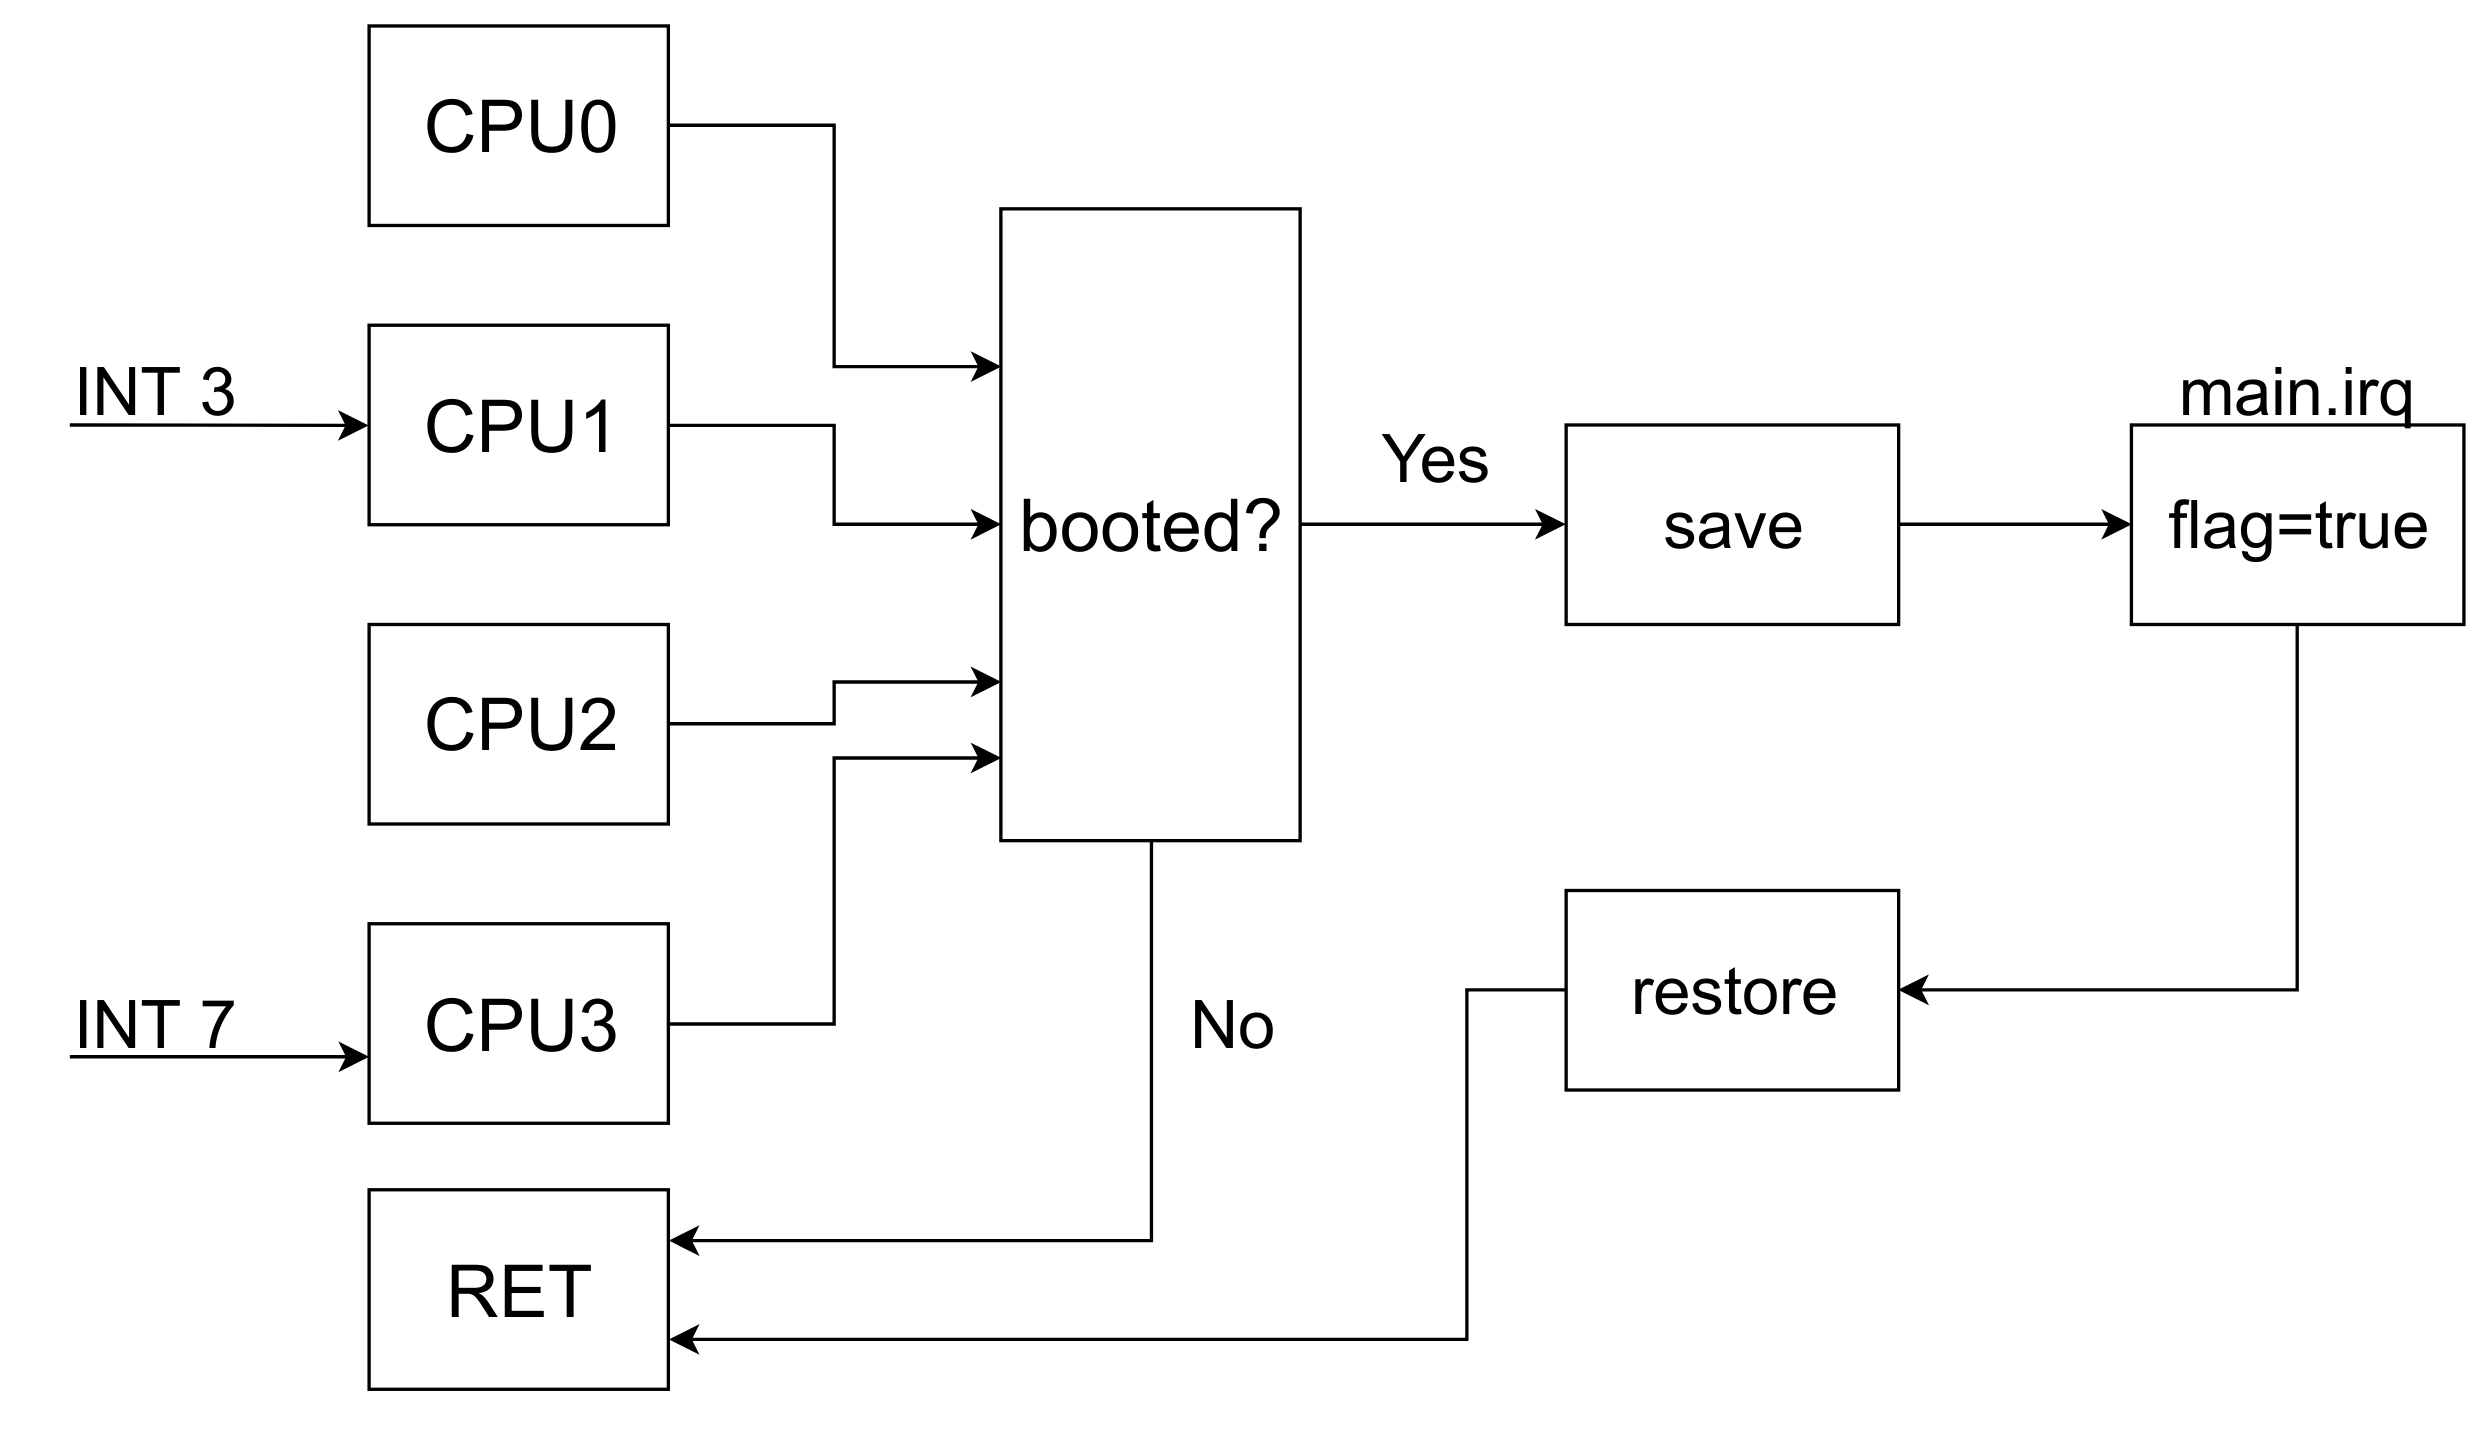
\includegraphics[scale=0.1]{interrupt}
\end{center}
  \caption{Handling Interrupts in GERT} \label{fig:interrupt}
\end{figure}

The interrupt handling process in GERT is explicitly designed so
that interrupts can always be serviced, even when Go's garbage collector
is running. To achieve this design, GERT puts some restrictions on the Go code
in an interrupt handler, as described below.

When a GC cycle runs, it can potentially stop the world and
prevent any Go code from executing. On a desktop OS it might be OK to disable
interrupts during a GC cycle because it is infrequent, but on an embedded system
interrupts could occur at any time, even while the world is
stopped. GERT allows interrupts to trigger at all times by assuming that the
interrupt handler does not perform any blocking operations. A block diagram
of the GERT interrupt process is shown in fig. \ref{fig:interrupt}.

GERT's interrupt handlers are written in Go and they execute on dedicated interrupt stacks.
When GERT receives an interrupt, the target processor
automatically switches its stack to the interrupt stack and then the GERT interrupt handler saves its old execution context onto the new stack.
Before proceeding any further, the interrupt handler checks a boolean flag to see if GERT has fully booted yet. This is important
for preventing unintentional Go code from executing while the memory map is still undefined.
While secretly executing on the interrupt stack, the processor can run any Go code
as long as it does not invoke the Go scheduler. This is because the Go runtime is unaware
of any interrupt code that can possibly run so it does not maintain any G's or M's to
run it. Thus, from the view of the Go runtime, the interrupt handler is running on an unknown secret stack which attaches itself
to whichever M was interrupted.

Interrupt handlers in GERT should not execute blocking operations or allocate memory from the Go heap \footnote{Go maintains a pool of free memory from which it allocates new objects. Most computer programs have a heap, not just Go programs.}.
The garbage collector is unaware of the hidden interrupt stacks so any heap-allocated objects on the stacks
will become memory leaks because the GC will never scan it. Fortunately, allocating heap objects in the interrupt
handler will cause a panic because \textit{make()}, and many other blocking operations, need to acquire
a lock from the runtime. This is dangerous because the runtime keeps track of which Ms are holding locks
and interrupt code can violate its beliefs and cause an unrecoverable panic.

Interrupt
routines should be short and execute quickly in order to avoid missing sequential
interrupts. This limits acceptable operations in an interrupt handler to toggling global boolean
flags and non-blocking reads/writes to memory. A typical GERT program is unaffected by these constraints
because it can use a goroutine to monitor a flag which is only toggled in the interrupt handler.

\subsection{Keeping Time}

Go needs a timer to schedule goroutines properly. GERT uses the 64bit ARM global timer which
is part of the general ARMv7a architecture \cite{ddi0406}. In the timer, each tick is about 2$ns$ so this means it will
not overflow for 1169 years. This means that GERT does not need a special timer interrupt to know when the
counter rolls over. The current value of the timer is returned whenever the Go runtime calls
the \textit{clock\_gettime()} syscall by reading from its MMIO address.

\subsection{Booting Secondary CPUs}

GERT boots auxiliary CPU's in two stages. After power on, the primary CPU starts executing at address 0x0 but the
secondary CPU's are held in a \textit{wait for interrupt} state. GERT creates an initial 4kb stack for each additional CPU,
which also doubles as its interrupt stack, before instructing them into a holding pen. The secondary CPU's
stay in the holding pen while GERT and the Go runtime finish booting because the virtual memory map is
in a state of flux. After GERT has booted, the user must call \textit{Release()} which causes the secondary CPU's
to reload their page tables and exit the holding pen into the GERT scheduler. Now the secondary CPU's
can each run Go threads normally.



\chapter{How to Use GERT}

It would be silly for this thesis to present a software toolkit and then
neglect to show how to use it.

\section{API Inspiration}
GERT's API is based on Arduino's because of its remarkable simplicity. In order to
get started with GERT on a Freescale iMX6 SOC, the programmer must only implement three functions: \textit{user\_init},
\textit{user\_loop} and \textit{irq}. \textit{user\_init} should contain code that is run only once
on startup, \textit{user\_loop} should contain the main event loop of the embedded program, and
\textit{irq} is the IRQ handler.

\section{Writing Interrupt Handlers}

Since interrupts can happen even while the world is stopepd, the programmer must make sure that \textit{irq} never executes
a blocking Go function or allocates memory on the Go heap with \textit{make()}. These constraints are
easily manageable by breaking the program interrupt logic into two pieces: a monitoring
goroutine which watches a boolean flag, and the interrupt service routine which sets the flag.
For example, a NIC driver may use interrupts to determine when a new frame should be retrieved
from the NIC. Rather than reading the new frame in the interrupt routine, the NIC driver
can set a flag in the interrupt routine so that a seperate thread inside the NIC driver can retrieve
the new frame. This seperate thread is just an ordinairy goroutine with no constraints on the type
of code it can execute.

\section{Building a GERT Program}

\begin{figure}[h]
\begin{center}
  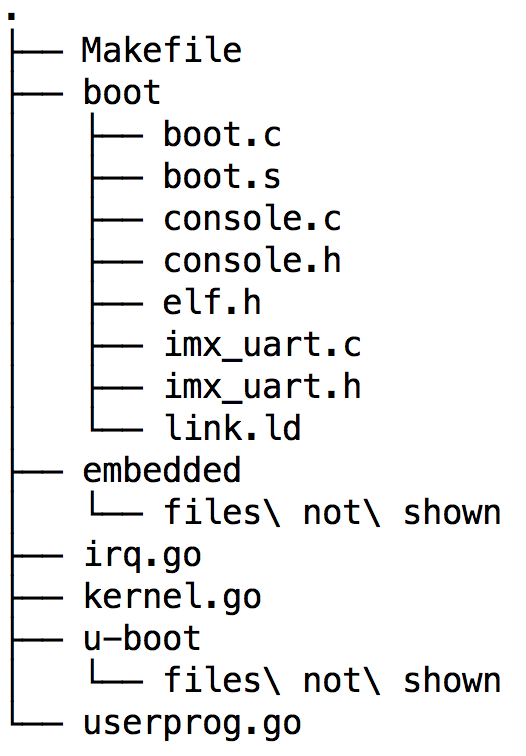
\includegraphics[scale=0.5]{dirtree}
\end{center}
  \caption{GERT Program Directory Layout} \label{fig:dtree}
\end{figure}

GERT needs a bootloader
and entry point to start on bare metal. The directory structure of a GERT
program is shown in fig. \ref{fig:dtree}. The boot directory contains the GERT
bootloader as well as linker script for it. Userprog.go and irq.go contain
the user-implemented functions as well as the user-implemented irq handler.
Kernel.go does three mundane things: it defines a new entry point for the Go runtime
(which just sets a flag so the runtime knows it is booting on bare metal),
it also finishes booting additional CPU's, and it configures the ARM Generic Interrupt Controller for normal operation. The makefile
is responsible for stitching the bootloader and GERT program together into an
sdcard image for u-boot. It uses \textit{go build} to build the GERT program
with the modified Go runtime and then it inserts the GERT program as a binary blob
into the boot loader's data section. The makefile also includes a target which writes
u-boot and the final GERT binary to an sdcard.

\section{Design Considerations}
Every SOC has a different memory map and peripherals, so GERT must be adjusted
accordingly. In order to change the link address of GERT, pass "-T <link address>"
as a link flag into \textit{go build}. The link address of the bootloader also needs
to be changed too inside link.ld. It is good practice to link the bootloader in an
area of RAM that can be reclaimed once GERT enables paging.

\section{Writing Drivers}
GERT imposes no driver model on the programmer. All drivers in
GERT should be written as normal Go code in the best style for
the intended application. GERT exposes no safe methods for reading
or writing device memory so any MMIO peripherals in the SOC must be
carefully programmed using the \textit{unsafe} package. Most MMIO
peripherals arrange their registers contiguously in memory so they
can be represented with a Go struct, which requires only one unsafe cast
for initial assignment.

GERT currently comes with an example driver
library in the form of a package called \textit{embedded}. The embedded package is not intrinsic to GERT's
functionality, nor was it optimized for performance in any way. The embedded package
just aims to provide a template for how drivers can be written in the Go language.
It only functions for the Freescale i.MX6 and includes drivers for the UART, SPI, PWM, GIC, USDHC, GPIO, and GPT peripherals.
The embedded package also includes a generic implementation of the FAT32 file system, which is
layered on top of a \textit{read} and \textit{write} function that the programmer can define.



%\include{chap2}
%% This is an example first chapter.  You should put chapter/appendix that you
%% write into a separate file, and add a line \include{yourfilename} to
%% main.tex, where `yourfilename.tex' is the name of the chapter/appendix file.
%% You can process specific files by typing their names in at the 
%% \files=
%% prompt when you run the file main.tex through LaTeX.
\chapter{Evaluation}

With GERT, the programmer should be able to implement concurrent embedded programs
which are as performant as the equivalent C implementation, but without having to
worry about concurency abstractions and memory safety bugs. In order to evaluate GERT,
there are two questions that must be answered:

\begin{enumerate}
  \item Does GERT retain good performance despite the costs of using a High Level Language?
  \item Do the concurrency patterns of Go simplify the task of the programmer?
\end{enumerate}

The first question is addressed by benchmarks below which measure GERT's
speed in creating and responding to external events. Pin toggle (\ref{sec:pin_toggle})
measures the maximum pin toggle frequency. Interrupt response time (\ref{sec:int_time})
measures the time it takes to respond to an external interrupt. Pulse counting
(\ref{sec:pulse_count}) counts number of pulses at increasing frequencies.
Concurrent response (\ref{sec:concurrent}) measures how many external events
GERT can concurrently respond to.

The second question is harder to answer because difficulty is a subjective
measure. This thesis attemps to show that GERT presents a better framework for
concurrency through two case studies: a robot sensor platform (\ref{sec:robot})
,which runs motors and reads sensors, and a galvo laser projector (\ref{sec:laser})
which traces images onto a surface by rotating mirrors at high speeds. The case studies
present a real-world experience for using GERT.

\section{Experimental Setup} \label{sec:setup}
In all tests, GERT is run on an i.MX6Quad SOC and all measurements are taken
with a Rigol DS1054Z oscilloscope. When GERT is compared to Linux, the SOC
runs Debian 8 "Jessie" with hardfloat support. GERT is also occasionally
compared to a Teensy 3.2 microcontroller running C. The Teensy 3.2 uses a Cortex M4, which is specifically
intended for microcontroller applications, and has good real-time performance. Its event
response times represent a good comparison point for GERT and Linux. The Teensy platform
has poor concurrency support though because its Cortex M4 is a single core processor.
%%and it only has 64 kilobytes of RAM.


All of the tests make use of the GERT "embedded" package, which is an example
driver library that was developed for the i.MX6Quad. The embedded package is not intrinsic to GERT's
functionality, nor was it optimized for performance in any way. The embedded package
just aims to provide a template for how drivers can be written in the Go language.
It currently includes drivers for the UART, SPI, PWM, GIC, USDHC, GPIO, and GPT peripherals.
The embedded package also includes an implementation of the FAT32 file system, which is 
currently unused.
%%used
%%for the laser projector (\ref{sec:laser}).

%%GERT is evaluated in conditions that are representative of embedded workloads.
%%The first few tests are benchmarks which measure GERT's maximum interrupt
%%frequency and pin toggle rate. The last two tests are each case studies: a robot
%%sensor platform and a scanning-mirror galvanometer laser projector. The test SOC
%%is the Freescale i.MX6Quad. Depending on the test, it is either running assembly,
%%GERT, or Debian 8 "Jessie" with hardfloat support. A Teensy 3.2 is used for comparison
%%on a few of the latency tests because of its Cortex M4 processor. All timing
%%measurements are taken using a Rigol DS1054Z oscilloscope.

\section{Pin Toggle Frequency}\label{sec:pin_toggle}
This test measures the speed at which GERT can toggle a simple GPIO pin on
the iMX6 Quad SOC. In ARM assembly, this can be implemented in 4 lines, but compilers and 
abstractions can increase the instruction count. Higher pin
toggling frequency indicates less code in the critical path.
GERT toggles the GPIO pin by directly interfacing with the GPIO
peripheral on the iMX6, but userspace Linux code must use the
sysfs driver.
Results are shown in figure \ref{fig:toggle}.


\begin{figure} [h]
\begin{center}
  \begin{tabular}{ | l | l |}
    \hline
    Platform & Avg GPIO Toggle Rate \\ \hline
    ASM & 1.65MHz \\ \hline
    GERT Static & 568KHz \\ \hline
    Linux C & 263KHz \\ \hline
    GERT & 154KHz \\ \hline
    Linux Go & 127KHz \\
    \hline
  \end{tabular}
\end{center}
  \caption{GPIO Toggle Rates of Different Platforms}  \label{fig:toggle}
\end{figure}

%%The results show that GERT does suffer a performance decrease because of
%%Go's abstraction cost but it is not clear why GERT underperforms user-space
%%Linux C code.
%%Without all of the syscalls a user-space program must endure, there should have
%%been a speed increase.

The results of the pin toggle initially show that GERT underperforms compared to
user-space Linux C. The reason became clear after tracing GERT's execution in QEMU:
the slowdown is caused by Go's interfaces in the embedded package. The GPIO driver
in the embedded package uses Go interfaces to abstract all of the different pins.
In order to toggle a single pin with an interface requires 47 instructions:
2 function calls, 19 loads, and 11 stores. In order to increase the toggle speed,
a new static GPIO driver was developed for GERT. The new driver is just a thin layer
over the memory-mapped registers. With static device ID's, the toggled pin
can be inferred at compile time instead of run time.
The performance of the static driver is also shown in the GERT static row
of figure \ref{fig:toggle}. With a static driver, GERT is able to toggle a
pin faster than user-space C code, but it is still very slow compared to
assembly.

But what if a Linux kernel module toggled the pin instead of userland code?
Pin toggle from inside a kernel module would certainly be faster than userland
C and it would also likely be faster than GERT. Operating from within
kernel space is very dangerous though because it lacks the protections that
GERT and userspace have.

\section{Interrupt Response Time}\label{sec:int_time}
This test measures the time it takes GERT to respond to an external event
with another external event. Specifically, it is the time it takes to produce
a rising edge on a GPIO pin in response to a falling edge on a different GPIO pin.
Faster response times are important for real time control systems, such as ABS brakes
in a car.
GERT and the Teensy detect the event with hardware interrupts
but Linux polls the input pin in a tight loop because the userspace sysfs
driver does not expose interrupt attachment points.
Results are shown below in figure \ref{fig:RT}.

\begin{figure} [h]
\begin{center}
  \begin{tabular}{ | l | l |}
    \hline
    Platform & Event Reponse Time \\ \hline
    Teensy 3.2 & 1$\mu$s \\ \hline
    GERT & 6.3$\mu$s \\ \hline
    Linux C & 10$\mu$s \\ \hline
    Linux Go & 30$\mu$s \\
    \hline
  \end{tabular}
\end{center}
  \caption{Event Response Times of Different Platforms}  \label{fig:RT}
\end{figure}

The event response times follow the increasing abstraction cost for each system.
The Teensy is very fast because its interrupt controller is vectored and interrupts
do not cause a stack switch. This means that the Teensy can flip a pin within a few cycles
of receiving the interrupt. GERT is slower because the iMX6 does not have a
vectored interrupt controller, the interrupt stack must be switched, and the
interrupt handler is written in Go. When GERT gets an interrupt, it must save its
current state, decide which interrupt it received, and execute its Go handler. Despite this
complexity, the iMX6 can execute more instructions in less time because of its very
high clock rate (792MHz vs 96MHz) so it can keep up with the Teensy.

The Linux configuration is slower because external interrupts cannot directly trigger a response
from userspace. In Linux, the GPIO pins are represented by file descriptors so
IO is performed by reading/writing from the appropriate file. In response to an external interrupt,
the Linux kernel sets a flag on the file descriptor which means that there is data to read. The userspace
program does not actually see the data until it is scheduled again.

As before, a Linux kernel module would likely attain the same performance as GERT
(or even more), but would lose the benefits of a HLL.


\section{Pulse Counting}\label{sec:pulse_count}
This test measures GERT's ability to count incoming pulses. Missed pulses
indicate an excessively long interrupt handler that is still executing when the next
pulse arrives. None of the platforms were configured for re-entrant interrupt handlers
so they can all potentially miss pulses.
The pulses are provided by a Xilinx Artix 7 FPGA and they are variable in
frequency and count. The Linux benchmarks are run with polling again because the
userspace sysfs driver does not support interrupt attachment.
Results are shown in figure \ref{fig:counter}.


\begin{figure} [h]
\begin{center}
  \begin{tabular}{ | l | l | l | l |}
    \hline
    Platform & Pulse Count & Max Pulse Rate & Missed Pulses \\ \hline
    Teensy 3.2 & 10 & 2.50MHz & 2 \\ \hline
    GERT & 10 & 161KHz & 1 \\ \hline
    Linux C & 10 & 161KHz & 4 \\ \hline
    Linux Go & 10 & 50KHz & 1 \\
    \hline
  \end{tabular}
\end{center}
  \caption{Pulse Counts of Different Platforms}  \label{fig:counter}
\end{figure}

GERT and userspace Linux C achieve similar performance on this test.
Linux just missed a few pulses.

The Teensy registers more pulses than any other platform because of its
compact and efficient architecture. A dissassembly of the Cortex M4 pulse count binary
reveals a fully vectorized interrupt whose routine only contains 5
instructions and zero conditional statements.

\section{Concurrent Events}\label{sec:concurrency}
Since the iMX6 has 4 cores, GERT should be able to concurrently
register 4 interrupts. The Teensy is configured to produce 10 rising edges
at 100KHz on a single pin and GERT must concurrently register them on 4 different
GPIO pins. The sum total of registered edges should be $10\times4=40$.

Because polling is a blocking operation, a multithreaded C program that concurrently
polls 4 pins is used for this test. The multithreaded C program is also compared
to a single-threaded C program. A multithreaded Go program which uses goroutines
to monitor pin states is also included.
Results are shown in figure \ref{fig:ccounter}.

\begin{figure} [h]
\begin{center}
  \begin{tabular}{ | l | l | l | l | l |}
    \hline
    Platform & Pulse Count & Pulse Rate & Min Registered & Max Registered \\ \hline
    GERT & 10 & 100KHz & 36 & 42 \\ \hline
    Linux C Multithread & 10 & 100KHz & 32 & 33 \\ \hline
    Linux C & 10 & 100KHz & 9 & 13 \\ \hline
    Linux Go & 10 & 100KHz & TBD & TBD \\
    \hline
  \end{tabular}
\end{center}
  \caption{Concurrent Pulse Counts of Different Platforms}  \label{fig:ccounter}
\end{figure}


<talk talk talk>

\section{Benchmark Conclusions}

Despite being written in a HLL, GERT can usually outperform userspace
Linux C code in the benchmarks that were conducted. GERT's performance trailed
Linux in the GPIO toggle test but, after changing the driver to a static model,
it also beat Linux in that test too. This is a promising result because it shows
that a HLL that provides the same isolations as a userspace can run on bare metal
and achieve higher performance.

Unlike Linux, GERT utilizes a true interrupt handler for delivering events.
In reality this doesn't seem to matter a lot because the latency difference
is still just a few microseconds.


GERT shows that it can usually outperform userspace Linux C code and it
can keep up with the Teensy in event response time. GERT also has a true interrupt
handler whereas Linux must poll due to the sysfs driver. Unfortunately, GERT
has a complicated interrupt pipeline with many conditionals so it can miss
more interrupts than the Teensy; GERT is not suitable for meeting hard deadlines.

GERT and Linux have similar concurrent capabilities. When the frequency of external
events exceeds the response time of a single core, the events can be split among
multiple cores. In GERT, though, this threshold frequency is about 4$\mu$s faster
so the programmer can avoid dedicating additional cores in some cases.


The Go garbage collector was never an issue during any of the tests because the
benchmark programs were all static. Without memory to reclaim, the GC never
had to run. However, if the GC did run, the only test that would have been affected is
the pin toggle test because the GC is allowed to stop the world. In GERT, interrupts
can trigger even when the world is stopped so the GC will not affect the response time
and pulse counting benchmarks even though it would affect them in the Linux Go benchmarks.

\section{Case Study: Robot Sensor Platform} \label{sec:robot}

\begin{figure}[h]
  \begin{center}
 \end{center}
  \caption{Code Breakdown of Robot Sensor Platform} \label{fig:robot_code}
\end{figure}

In order to evaluate GERT on a realistic workload, I put it on a robot that was
donated to me from MIT's MASLAB competition. Among other things, the robot has two drive
motors with encoders and also several Sharp GP2Y0A21YK infrared distance sensors on its perimeter.
I wrote a program in Go using GERT to process all of these event sources at the same time
and operate the robot.

\subsection{Overview}
The main body of the robot program is an event loop which waits for events coming out of an event channel (fig. \ref{fig:event_loop}).
Independent goroutines monitor each sensor and send events into the event channel. There is a
single goroutine that monitors the event channel and manipulates state in a non-blocking manner. The code for the
event loop is shown below in fig. \ref{fig:event_loop}.

\begin{figure}[h]
  \begin{center}
\begin{lstlisting}
select {
	case event := <-event_chan:
		fmt.Printf("%v\n", event)
		switch event {
		case "p":
			val := adc.Read(0)
			fmt.Printf("adc reads %v\n", val)
		case "w":
			drive.Forward(0.2)
		case "s":
			drive.Backward(0.2)
		case "a":
			drive.TurnRight(0.2)
		case "d":
			drive.TurnLeft(0.2)
		case " ":
			drive.Stop()
		}
	}
\end{lstlisting}
\end{center}
  \caption{Robot Event Loop} \label{fig:event_loop}
\end{figure}

The robot program uses Go's higher order functions and closures in order to create a sensor polling helper function
as shown below in fig. \ref{fig:poll_func}. In this paradigm, every sensor gets its own goroutine which sends
data back into a central event loop.

%%\clearpage

\begin{figure}[!h]
\begin{center}
\begin{lstlisting}
type Pollfunc func() interface{}

func Poll(f Pollfunc, period time.Duration,
sink chan interface{}) chan bool {
	kill := make(chan bool)
	go func(kill chan bool) {
		for {
			select {
			case <-kill:
				return
			default:
				if period > 0 {
					time.Sleep(period)
				}
				sink <- f() //sink is usually the event channel
			}
		}
	}(kill)
	return kill
}
\end{lstlisting}
\end{center}
  \caption{Higher Order Polling Function} \label{fig:poll_func}
\end{figure}

The robot program also configured the GPIO library to use interrupts in order to count pulses on the encoder (fig. \ref{fig:encoder}).

\begin{figure}[!h]
\begin{center}
\begin{lstlisting}
embedded.WB_JP4_10.SetInput()
embedded.WB_JP4_10.EnableIntr(embedded.INTR_FALLING)
embedded.Enable_interrupt(99, 0) //send GPIO1 interrupt to CPU0
.
//go:nosplit
//go:nowritebarrierec
func irq(irqnum uint32) {
	switch irqnum {
...
	case 99:
		inc()
		embedded.ClearIntr(1)
...
	}
}
.
func inc() {
	count += 1
}

\end{lstlisting}
\end{center}
  \caption{Encoder Interrupt} \label{fig:encoder}
\end{figure}

With these powerful set of abstractions, adding events or sensors into the event loop
is simple because only a Pollfunc() must be implemented. As an added bonus, this
GERT program is automatically concurrent because the Go and GERT schedulers will
move idle cpus to any available goroutine. The rest of this case study explains how the sensors
are interfaced with GERT.


\subsection{PWM Motor Control}
The robot has an MDD10A motor speed controller for controlling the two drive motors. This device
expects a pulse-width modulated signal (PWM) on its input pins in order to direct power into the
motors. A PWM signal has a constant period and the signal is a logical "on" for part of the time
and "off" for the rest of the time (fig. \ref{fig:pwm}). The ratio of "on" time vs the period is called the duty cycle.
It is this percentage which the motor controller translates into a speed for the motor.

\begin{figure}[h]
\begin{center}
  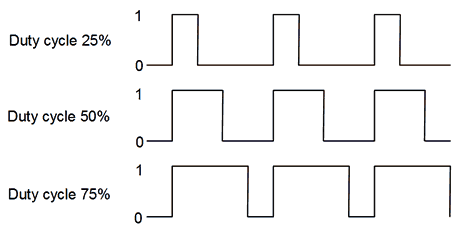
\includegraphics[scale=0.5]{pwm}
\end{center}
  \caption{Sample PWM Signals} \label{fig:pwm}
\end{figure}


The iMX6Q includes an on-board PWM peripheral which can output several channels of PWM
at a variety of periods and duty cycles. GERT contains a driver for this PWM peripheral in its embedded
package. The PWM peripheral requires no maintenance once it is configured so the cost of outputting
a PWM signal is essentially a few loads and stores every time the user changes the period or duty cycle.

The driver is organized in a typical C fashion where the memory map of the peripheral is represented in a structure:
\begin{figure}[h]
  \begin{subfigure}[t!]{0.5\textwidth}
  \begin{lstlisting}
  type PWM_regs struct {
	CR  uint32
	SR  uint32
	IR  uint32
	SAR uint32
	PR  uint32
	CNR uint32
}
  \end{lstlisting}
  \end{subfigure}
  \begin{subfigure}[t!]{0.5\textwidth}
 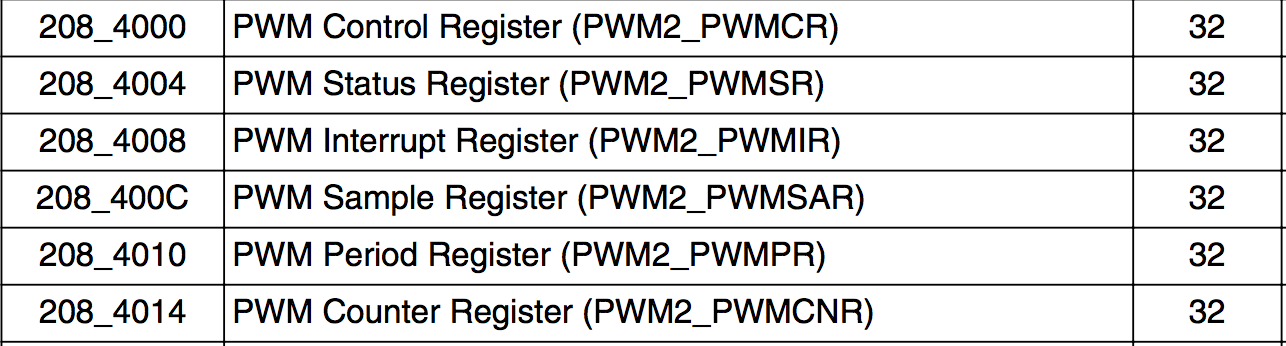
\includegraphics[scale=0.4]{pwmregs}
  \end{subfigure}
  \caption{PWM Register Representation} \label{fig:pwm_struct}
\end{figure}

The driver also exposes methods for stopping. starting, and setting the
frequency and duty cycle of the PWM generator:
\begin{figure}[h]
  \begin{lstlisting}
func (pwm *PWM_periph) Begin(freq khz)
func (pwm *PWM_periph) Stop()
func (pwm *PWM_periph) SetFreq(freq khz)
func (pwm *PWM_periph) SetDuty(dutycycle float32)
  \end{lstlisting}
  \caption{PWM Driver API} \label{fig:pwm_api}
\end{figure}

\subsection{Distance Sensor Reading}
The Sharp distance sensor outputs an analog voltage proportional to its distance from the nearest object (fig. \ref{fig:curve}).
A Microchip MCP3008 8-channel ADC is used to convert this voltage into a digital signal. The MCP3008 communicates in clocked
serial (SPI) with 24bit data frames so the robot program uses GERT's SPI driver. Much like the
PWM peripheral, the SPI peripheral has multiple channels that can each concurrently send and receive data. The SPI
driver also requires no input from the user except for the data to transmit and receive.

\begin{figure}[h]
\begin{center}
  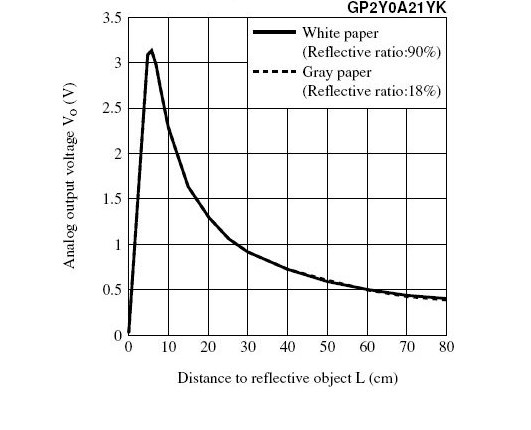
\includegraphics[scale=0.5]{IRSensor-3}
\end{center}
  \caption{Sharp Sensor Distance Curve} \label{fig:curve}
\end{figure}

\clearpage
\subsection{Encoder Reading}
Encoders emit a pulse every time the motor rotates a known amount. This amount is variable depending on the
encoder resolution. The encoders on the test motors emit pulses at a max rate of 4KHz, corresponding to
maximum motor speed. GERT had no difficulty picking up these pulses because this frequency is far less than
the max pulse frequency in fig. \ref{fig:counter}. A speed monitor was written in fig. \ref{fig:speedmon}
to measure the motor rotation (in Hz) and it corresponded very closely to the oscilliscope readings.

\begin{figure}[h]
\begin{center}
\begin{lstlisting}
//count is updated by the interrupt routine
//and it is the amount of encoder pulses
go func() {
  for {
    old := count
    time.Sleep(1 * time.Second)
    new := count
    event_chan <- new - old
  }
}()
\end{lstlisting}
\end{center}
  \caption{Motor Speed Monitor} \label{fig:speedmon}
\end{figure}

\subsection{Complications}
Systems do not work perfectly, and this robot is no exception. The switching motor controller used
on this robot emits a lot of noise. The 5v noise spikes measured on the oscilloscope wreaked havoc
on the 3.3v single-ended signals that the iMX6 operates with, causing serial communication failures
and spurious interrupts. To deal with this, the robot's motors are connected to an external power supply before
taking measurements. This helps remove noise from the digital circuits. Consequently, the physical
robot cannot move when the motors are connected to an external power supply.

\subsection{Result}
GERT is a plausible embedded toolkit to use for robots that incorporate many sensor systems.
By utilizing Go's language features, an embedded firmware engineer can implement a complicated sensor integration
platform on top of GERT without worrying about issues like scheduling or shared memory. The robot sensor platform
never experienced a single use-after-free, index out of range, or memory safety bug because it is implemented in a HLL.
As an added bonus, the robot sensor platform also does not contain a single lock despite the fact that every sensor
runs in its own thread, deadlock will never occur.



\section{Case Study: Laser Projector}\label{sec:laser}
A scanning-mirror galvanometer laser projector is a device that deflects a laser beam off of several mirrors in
order to draw an image on another surface, as shown in fig. \ref{fig:galvos}. If the entire image can be scanned faster than 24Hz, then the light appears
to blend and the human brain perceives it as a single image rather than many points. The maximum rate at which the
projector can trace points is bounded below by the speed of the galvos and bounded above by the speed of the software.
In this case study, GERT is used to implement a laser projector with a red laser.

\begin{figure}[h]
\begin{center}
  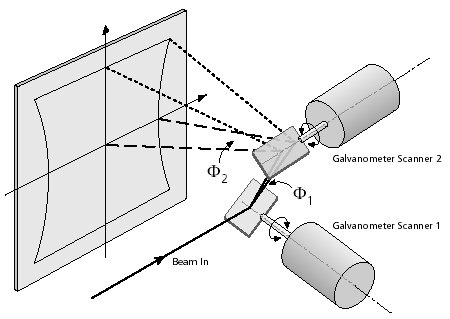
\includegraphics[scale=0.5]{galvanometer}
\end{center}
  \caption{Mirror Galvanometers} \label{fig:galvos}
\end{figure}

\subsection{Overview}
Points are generated from a vector graphics file on a desktop computer and stored
on an sdcard before GERT loads them and traces the image. The laser projector,
unlike the robot sensor platform, does not have to process any external events or
manage concurrency.
Instead, the laser program must just be fast enough to trace points smoothly.
To do this, GERT runs a dedicated goroutine, $lasermon$ which loops over all of the points
in a circular buffer and sends them in order to a Microchip MCP4922 DAC. The
DAC converts the digital position signal into an analog voltage and then
sends that voltage signal into an analog servo circuit, which sets the position
of the mirrors.

\subsection{Point Serialization}
The laser program uses Go's native Gob library in order to serialize and
deserialize points. The laser projector is currently limited to
two dimensional images with a single red laser, so only three
properties must be stored for each point: X position, Y position,
and Color. The DAC only has a 12bit resolution so 16bit integers are used
to store each point. The struct is shown below in fig. \ref{fig:cpoint}

\begin{figure}[!h]
\begin{center}
\begin{lstlisting}
type CompactPoint struct {
	X     uint16
	Y     uint16
	Color uint8 //either 0 or 1
}
\end{lstlisting}
\end{center}
  \caption{Laser Point Structure} \label{fig:cpoint}
\end{figure}

In order to store points, a seperate encoding program running
on a desktop computer encodes an array of $CompactPoint$ structs into
a Gob object and writes them to a file. Next, the encoding program stores
the file onto the FAT32-formatted sdcard that contains the GERT
program. Then, GERT reads the same file and de-serializes the Gob object
into an array of $CompactPoint$, like in fig. \ref{fig:loadpoints}.

\begin{figure}[!h]
\begin{center}
\begin{lstlisting}
	good, root := embedded.Fat32_som_start(embedded.Init_som_sdcard,
  embedded.Read_som_sdcard)
	if !good {
		fmt.Println("fat32 init failure")
	}
	good, bootdir := root.Direnter("BOOT")
	if !good {
		panic("dir entry failed")
	}
  /* P.TXT contains the Gob'ed points */
	good, contents := bootdir.Fileread("P.TXT")
	if !good {
		panic("file read failure")
	}
	r := bytes.NewBuffer(contents)
	d := gob.NewDecoder(r)
	err := d.Decode(&points)
	if err != nil {
		fmt.Printf("error de-GOBing:\n")
		panic(err)
	}
\end{lstlisting}
\end{center}
  \caption{Laser Point Structure} \label{fig:loadpoints}
\end{figure}



\appendix
%\chapter{Tables}

\begin{table}
\caption{Armadillos}
\label{arm:table}
\begin{center}
\begin{tabular}{||l|l||}\hline
Armadillos & are \\\hline
our	   & friends \\\hline
\end{tabular}
\end{center}
\end{table}

\clearpage
\newpage

%\chapter{Figures}

\vspace*{-3in}

\begin{figure}
\vspace{2.4in}
\caption{Armadillo slaying lawyer.}
\label{arm:fig1}
\end{figure}
\clearpage
\newpage

\begin{figure}
\vspace{2.4in}
\caption{Armadillo eradicating national debt.}
\label{arm:fig2}
\end{figure}
\clearpage
\newpage

%%% This defines the bibliography file (main.bib) and the bibliography style.
%% If you want to create a bibliography file by hand, change the contents of
%% this file to a `thebibliography' environment.  For more information 
%% see section 4.3 of the LaTeX manual.
\begin{singlespace}
\bibliography{main}
\bibliographystyle{plain}
\end{singlespace}

\end{document}

